\documentclass[11pt]{article}
\usepackage[utf8]{inputenc}
\usepackage[margin=1in]{geometry}
\usepackage{siunitx,pgfplots,fancyhdr,enumitem,tikz,xparse,listings,graphicx}

%%Needed to properly display graphs
\pgfplotsset{width=10cm,compat=1.9}

\pagestyle{fancy}
\fancyhf{}
\lhead{Steven Glasford}
\chead{Homework 1}
\rhead{Page \thepage}

\title{Homework 1}
\author{Steven Glasford}
\date{\parbox{\linewidth}{\centering%
    %%Adds the last compiled date
    \today\endgraf\medskip
    Numerical Analysis\endgraf\medskip
    MATH-373}}

%%Creates a new symbol for plus and minus together
\newcommand{\rpm}{\sbox0{$1$}\sbox2{$\scriptstyle\pm$}
  \raise\dimexpr(\ht0-\ht2)/2\relax\box2 }

%%Creates a nice format for displaying the steps taken  
\newlist{steps}{enumerate}{1}
\setlist[steps, 1]{label = Step \arabic*:}

\ExplSyntaxOn
%%new command to round numbers
\newcommand*{\prlen}[1]{%
   % round to 1 digit:
    \pgfmathparse{round(10)/10.0}%
    %\pgfkeys{/pgf/number format/precision=1}
    %\pgfmathresult
    \pgfmathprintnumber[fixed, precision=2]{\pgfmathresult}
}
\ExplSyntaxOff

% Set the listings programming language
\lstset{language=Matlab}

\begin{document}

%% adds the title to the document
\maketitle
\pagebreak
%\tableofcontents

\section{Problem Statement}
Solve the secant formula, $\sigma_{max} = \frac{P}{A}\left(1+\epsilon_r sec \left( \left(\frac{L}{2k}\right)\sqrt{\frac{P}{EA}}\right)\right)$ using the methods of Bisection and False Position.
\section{Solution}

If $\sigma_{max} = 200,000 $MPa/m$^2$ is the maximum stress for the material used to make the column, $\epsilon_r$ is the eccentricity ratio, $E=150000$ MPa is the modulus of elasticity, and $L/k = 30$ is the slenderness ratio, then determine the smallest stress, $P/A$

\begin{center}
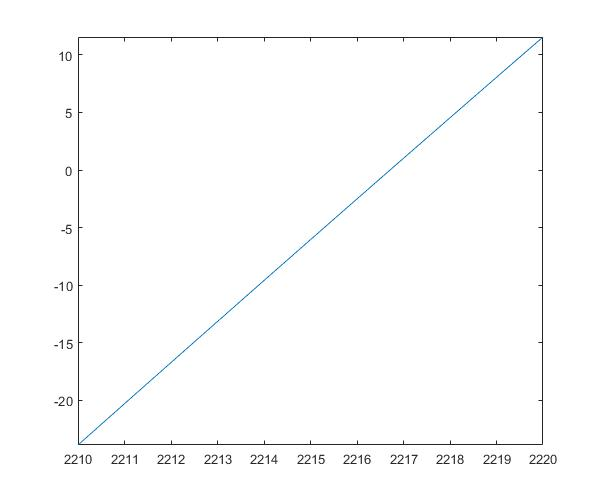
\includegraphics[scale=.5]{secant.jpg}
\end{center}
Before I was able to figure out where the bounds of the graph should be I graphed it using the online graphing calculator Desmos to get a rough idea of where to bound it. I decide that the interval 2210 and 2220 was a decent range.

results in data as follows:

\begin{table}[h]
\begin{center}
\caption{Results from Bisection and False Position.}\label{table:kepler}
\smallskip
\begin{tabular}{l|cccc}
Method & \texttt{x\_root} & \texttt{func\_val} & $\varepsilon_a$ & Iterations\\\hline
Bisection & \num{2216.7} & \num{-0.0028} & \num{6.6082e-05} & 14\\
False Position & 2216.7 & \num{2.0595e-05} & \num{1.2455e-05} & 3\\
\end{tabular}
\end{center}
\end{table}

It seemed that the false-position method was faster.

\section{Command-line Usage}
One program was written to solve this problem, and the command-line usage is below.

\begin{verbatim}
>> secant()
\end{verbatim}

\section{Code}

A program was written to solve this problem, called \texttt{secant}, and the code can be found in Listing \ref{code:problem}.

Also included is \texttt{bisection} and \texttt{false_position} which is found at 

\begin{lstlisting}[caption={MATLAB code for solving secant eqaution.}, label = {code:problem},frame=tb]
%%%%%%%%%%%%%%%%%%%%%%%%%%%%%%%%%%%%%%%%%%%%%%%%%%%%%%%%%%%%%%%% 
%Steven Glasford
% Febuary 1, 2018
% Plot the Secant Formula 

% No inputs

% No Outputs. Plots are automatically generated
%%%%%%%%%%%%%%%%%%%%%%%%%%%%%%%%%%%%%%%%%%%%%%%%%%%%%%%%%%%%%%%

% Constants
function secant()
secant_func = @(x) x*(1+.25*sec((30/2)*sqrt(x/150000)));
fplot(secant_func);

fplot(secant_func,[2210 2220])
x_min = 2201;
x_max = 2249;
[bi_root,bi_func_val,bi_error_approx,bi_num_iterations] = bisection(...
    secant_func,x_min,x_max)
[falseroot,falsefunc_val,falseerror_approx,falsenum_iterations] = ...
    false_position(secant_func,x_min,x_max)

end
\end{lstlisting}

\begin{lstlisting}[caption={MATLAB code for bisection}, label = {code:bisection},frame=tb]
%%%%%%%%%%%%%%%%%%%%%%%%%%%%%%%%%%%%%%%%%%%%%%%%%%%%%%%%%%%%%
% Steven Glasford
% Febuary 1, 2018
% implement bisection 

% inputs:  func, x_min, x_max, error_desired, max_iterations

% outputs: root, func_val, error_approx, num_iterations
%%%%%%%%%%%%%%%%%%%%%%%%%%%%%%%%%%%%%%%%%%%%%%%%%%%%%%%%%%%%%%%%

function [root,func_val,error_approx,num_iterations] = bisection(func,...
    x_min,x_max,error_desired,max_iterations)

%check inputs and assign defaults

%Requires more than 3 entries for the function to work
if (nargin < 3)
    error('At least three arguments are required');
end

if ((nargin < 4) || isempty(error_desired))
    error_desired = .0001;
end

if ((nargin < 5) || isempty(max_iterations))
    max_iterations = 50;
end

error_approx=100;
x_bar_old=x_min;
x_bar_new=x_min;
num_iterations=0;

while (error_desired<error_approx && num_iterations < max_iterations)
    
    x_bar_old=(x_min + x_max)/2;
    test = func(x_min)*func(x_bar_old);
    
    if (test < 0)
        x_max = x_bar_old;
           
    elseif (test > 0)
        x_min = x_bar_old;
        
    else
        root = x_bar_old;
        error_approx = 0;
        break
    end
    
    x_bar_new = (x_max + x_min)/2;
    
    if (x_bar_new ~= 0)
            error_approx = abs((x_bar_new - x_bar_old)/x_bar_new)*100;
    end 
    num_iterations = num_iterations + 1;
end

func_val = func(x_bar_new);
root = x_bar_new;

end
\end{lstlisting}

\begin{lstlisting}[caption={MATLAB code for false_position}, label = {code:false},frame=tb]
%%%%%%%%%%%%%%%%%%%%%%%%%%%%%%%%%%%%%%%%%%%%%%%%%%%%%%%%%%%%%%%%%
% Steven Glasford
% Febuary 1, 2018
% false position implementation 

% inputs:  func, x_min, x_max, error_desired, max_iterations

% outputs: root, func_val, error_approx, num_iterations
%%%%%%%%%%%%%%%%%%%%%%%%%%%%%%%%%%%%%%%%%%%%%%%%%%%%%%%%%%%%%%%%%


function [root,func_val,error_approx,num_iterations] = false_position(...
    func,x_min,x_max,error_desired,max_iterations)

%check inputs and assign defaults

%Requires more than 3 entries for the function to work
if (nargin < 3)
    error('At least three arguments are required');
end

if ((nargin < 4) || isempty(error_desired))
    error_desired = .0001;
end

if ((nargin < 5) || isempty(max_iterations))
    max_iterations = 50;
end

error_approx=100;
x_r_old=x_min;
x_r_new=x_min;
num_iterations=0;

while (error_desired<error_approx && num_iterations < max_iterations)
    
    x_r_old = x_max - (func(x_max) * (x_min - x_max))/(func(x_min) - ...
        func(x_max));
    
    test = func(x_min)*func(x_r_old);
    
    if (test < 0)
        x_max = x_r_old;
           
    elseif (test > 0)
        x_min = x_r_old;
        
    else
        root = x_r_old;
        error_approx = 0;
        break
    end
    
    x_r_new = x_max - (func(x_max) * (x_min - x_max))/(func(x_min) - ...
        func(x_max));
    
    if (x_r_new ~= 0)
            error_approx = abs((x_r_new - x_r_old)/x_r_new)*100;
    end 
    num_iterations = num_iterations + 1;
end

func_val = func(x_r_new);
root = x_r_new;

end
\end{lstlisting}

\end{document}